\chapter{Boards} \hypertarget{def:boards}{}

PICSimLab currently supports five backend simulators. The stable version supports 
\href{https://github.com/lcgamboa/picsim}{picsim} and \href{https://github.com/buserror/simavr}{simavr}. 
The experimental version supports \href{http://mazsola.iit.uni-miskolc.hu/\%7edrdani/embedded/ucsim/}{uCsim}, 
\href{http://gpsim.sourceforge.net/}{gpsim} and \href{http://beckus.github.io/qemu_stm32/}{qemu-stm32} in 
addition to the stable ones.

The Figure below shows which cards are based on which backend simulator:

\begin{figure}[H] 
\center
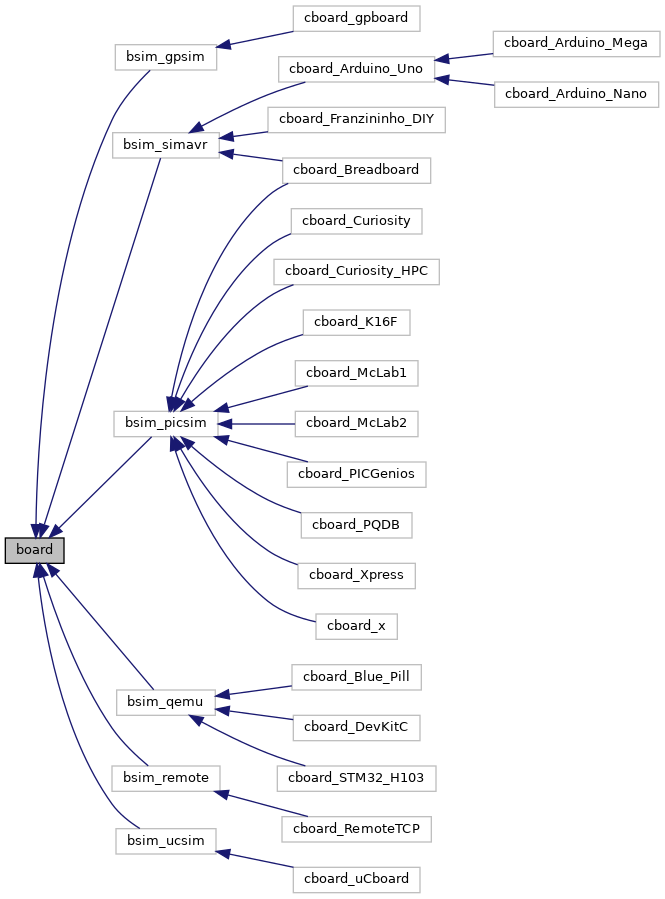
\includegraphics[width=0.65\textwidth]{img/boards.png} 
\caption{Boards backend simulators}
\end{figure} 

The below table show the supported debug interface of each simulator:

\begin{center}
\begin{tabular}{c|c}
\hline \textbf{Backend} & \textbf{Debug Support}\\
\hline picsim & see the section \hyperlink{def:mplabxd}{MPLABX Integrated Debug}\\
\hline simavr & see the sections \hyperlink{def:mplabxd}{MPLABX Integrated Debug} and \hyperlink{def:gdbavr}{remote avr-gdb Debug}\\
\hline qemu-stm32 & see the section \hyperlink{def:gdbarm}{remote arm-gdb Debug}\\
\hline uCsim & see the section \hyperlink{def:ucsim}{uCsim remote console (telnet) Debug}\\
\hline gpsim & none yet\\
\hline 
\end{tabular}
\end{center}



\section{Breadboard}

It is a generic board only with reset, serial and crystal circuits and support to multiple microcontrollers 
of \href{https://github.com/lcgamboa/picsim}{picsim} and \href{https://github.com/buserror/simavr}{simavr}.

\begin{figure}[H]
\center
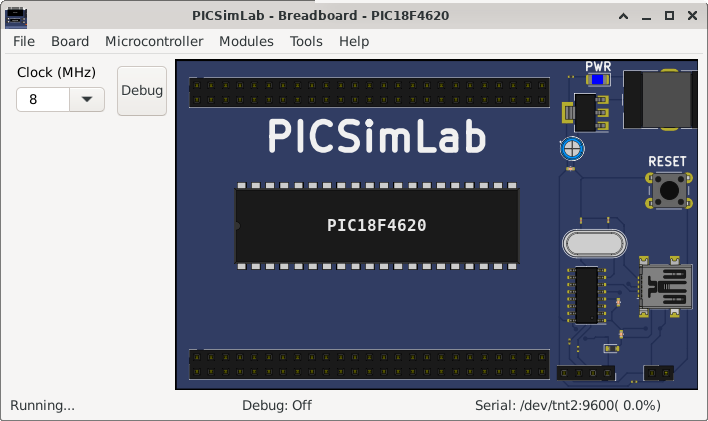
\includegraphics[width=0.7\textwidth]{img/picsimlab0.png} 
\end{figure} 

\href{https://lcgamboa.github.io/picsimlab_examples/board_Breadboard.html}{Examples}

\section{McLab1}

It emulates the Labtools development board McLab1 that uses one PIC16F84, PIC16F628 or PIC16F648 of \href{https://github.com/lcgamboa/picsim}{picsim}.

\begin{figure}[H]
\center
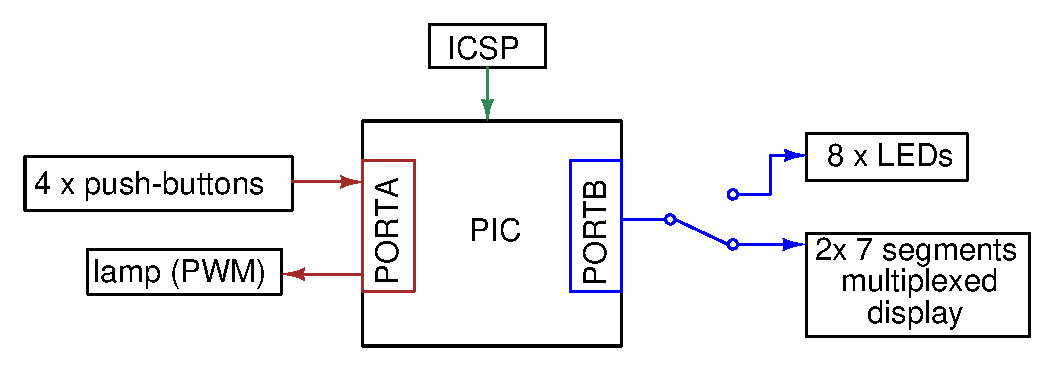
\includegraphics[width=0.85\textwidth]{img/blocks_p1.eps} 
\end{figure} 


\begin{figure}[H]
\center
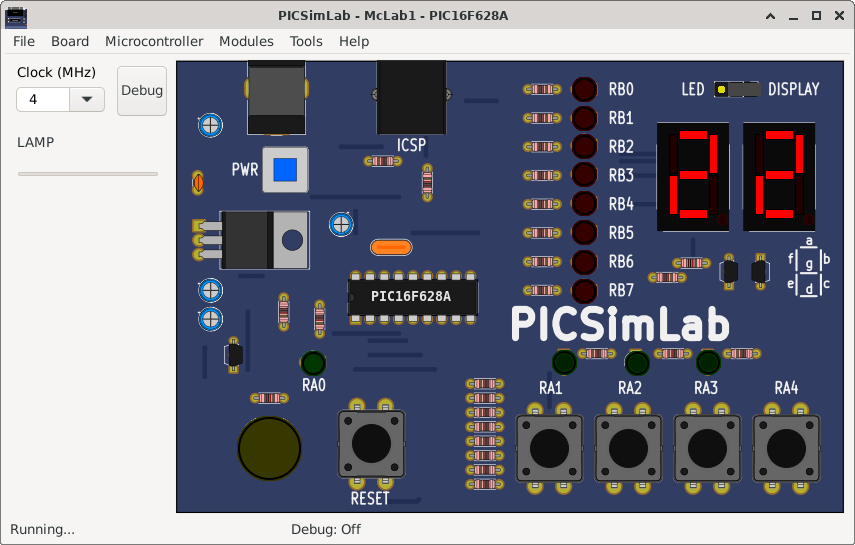
\includegraphics[width=0.7\textwidth]{img/picsimlab1.png} 
\end{figure} 

\hrefb{pdf/board1.pdf}{Board McLab1 schematics}.\vspace{0.5cm}

The code examples can be loaded in PICSimLab menu \textbf{Help->Examples}.

The source code of board McLab1 examples using \href{http://www.microchip.com/mplabx}{MPLABX and XC8} compiler 
are in the link: \href{https://lcgamboa.github.io/picsimlab_examples/board_McLab1.html}{board\_McLab1}.

\section{K16F}

It emulates an didactic board developed by author that uses one PIC16F84, PIC16F628 or PIC16F648 of \href{https://github.com/lcgamboa/picsim}{picsim}.

\begin{figure}[H]
\center
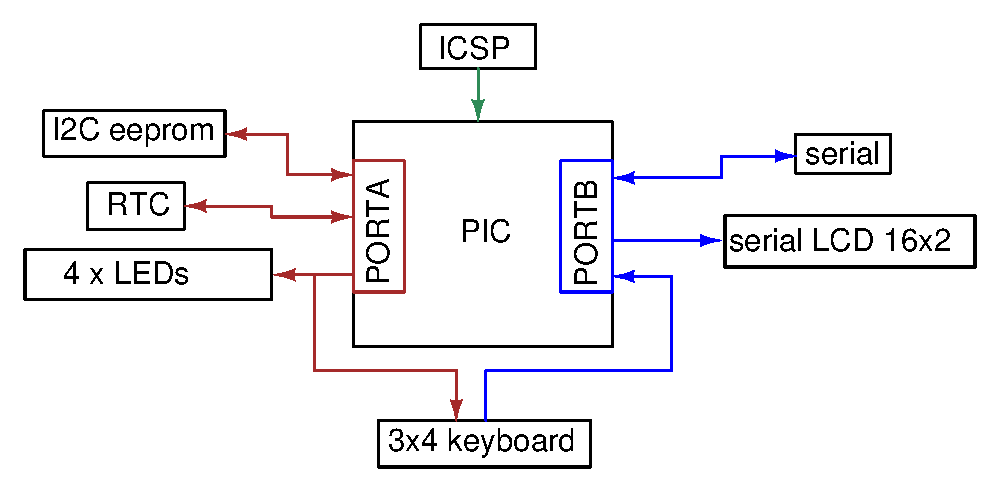
\includegraphics[width=0.85\textwidth]{img/blocks_p2.eps} 
\end{figure} 


\begin{figure}[H]
\center
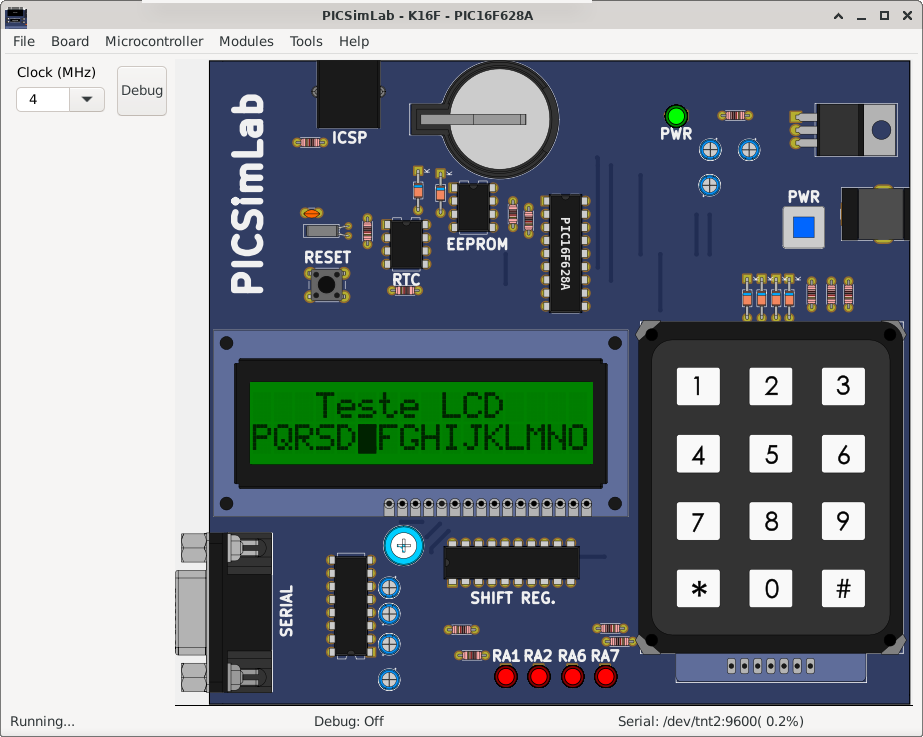
\includegraphics[width=0.8\textwidth]{img/picsimlab2.png} 
\end{figure} 

\hrefb{pdf/board2.pdf}{Board K16F schematics}.\vspace{0.5cm}

The code examples can be loaded in PICSimLab menu \textbf{Help->Examples}.

The source code of board K16F examples using \href{http://www.microchip.com/mplabx}{MPLABX and XC8} compiler are in
the link: \href{https://lcgamboa.github.io/picsimlab_examples/board_K16F.html}{board\_K16F}.


\section{McLab2}

It emulates the Labtools development board McLab2 that uses one PIC16F777, PIC16F877A, PIC18F452, PIC18F4520, PIC18F4550 or PIC18F4620 of \href{https://github.com/lcgamboa/picsim}{picsim}.

\begin{figure}[H]
\center
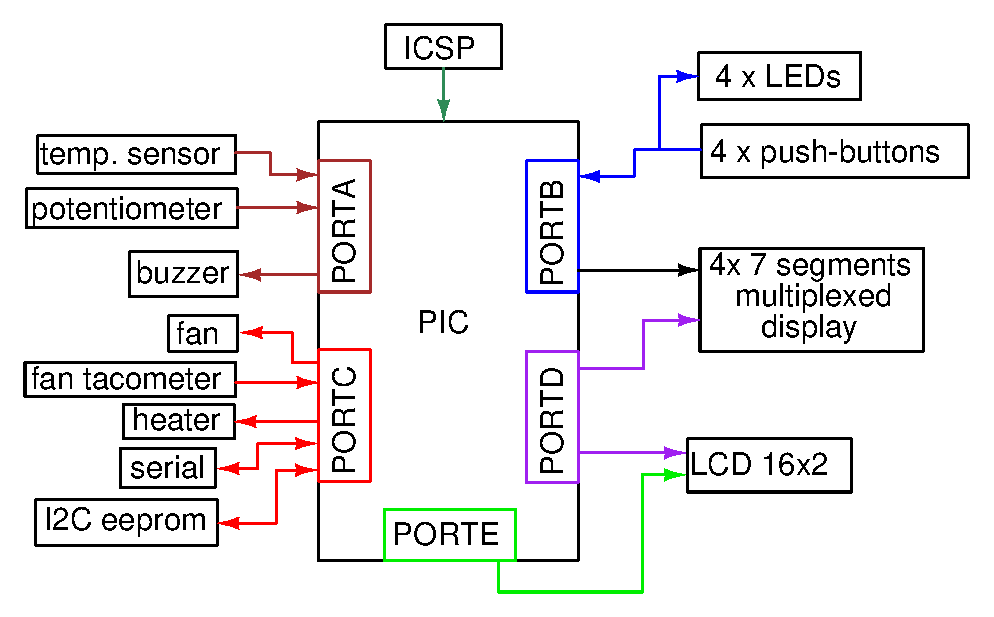
\includegraphics[width=0.85\textwidth]{img/blocks_p3.eps} 
\end{figure} 


\begin{figure}[H]
\center
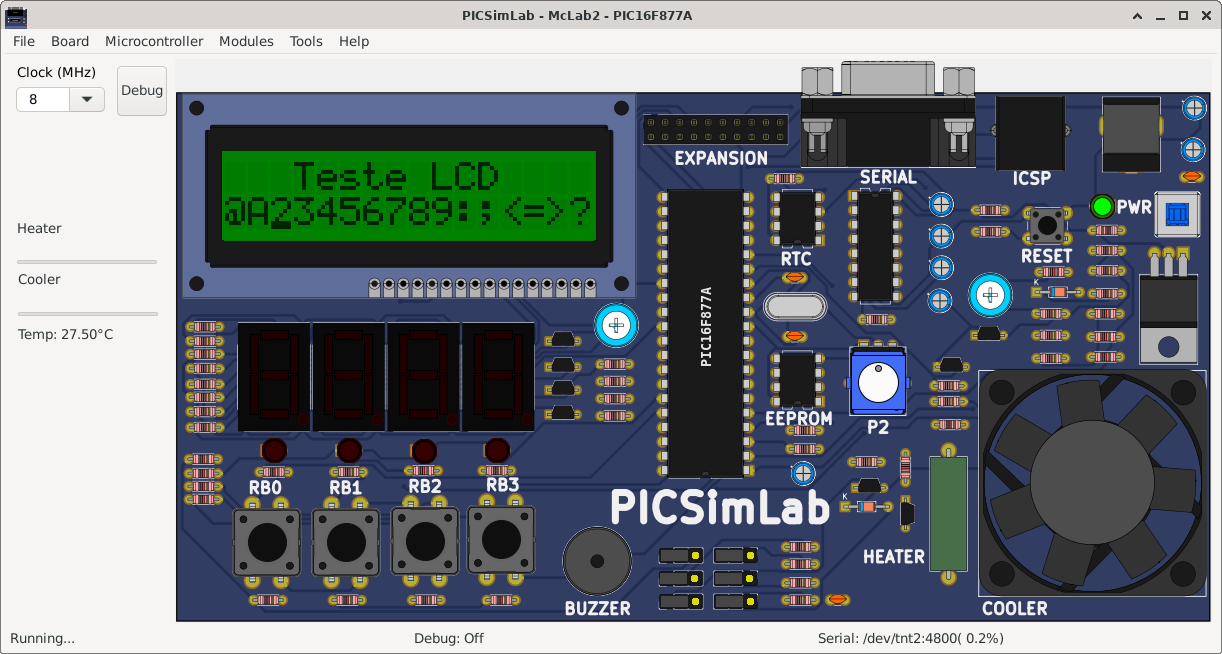
\includegraphics[width=0.9\textwidth]{img/picsimlab3.png} 
\end{figure} 

\hrefb{pdf/board3.pdf}{Board McLab2 schematics}.\vspace{0.5cm}

The code examples can be loaded in PICSimLab menu \textbf{Help->Examples}.

The source code of board McLab2 examples using \href{http://www.microchip.com/mplabx}{MPLABX and XC8} 
compiler are in the link: \href{https://lcgamboa.github.io/picsimlab_examples/board_McLab2.html}{board\_McLab2}.

\section{PICGenios}

It emulates the microgenius development board PICGenios PIC18F e PIC16F Microchip that uses one PIC16F777, PIC16F877A, PIC18F452, PIC18F4520, PIC18F4550 or PIC18F4620 of \href{https://github.com/lcgamboa/picsim}{picsim}.

\begin{figure}[H]
\center
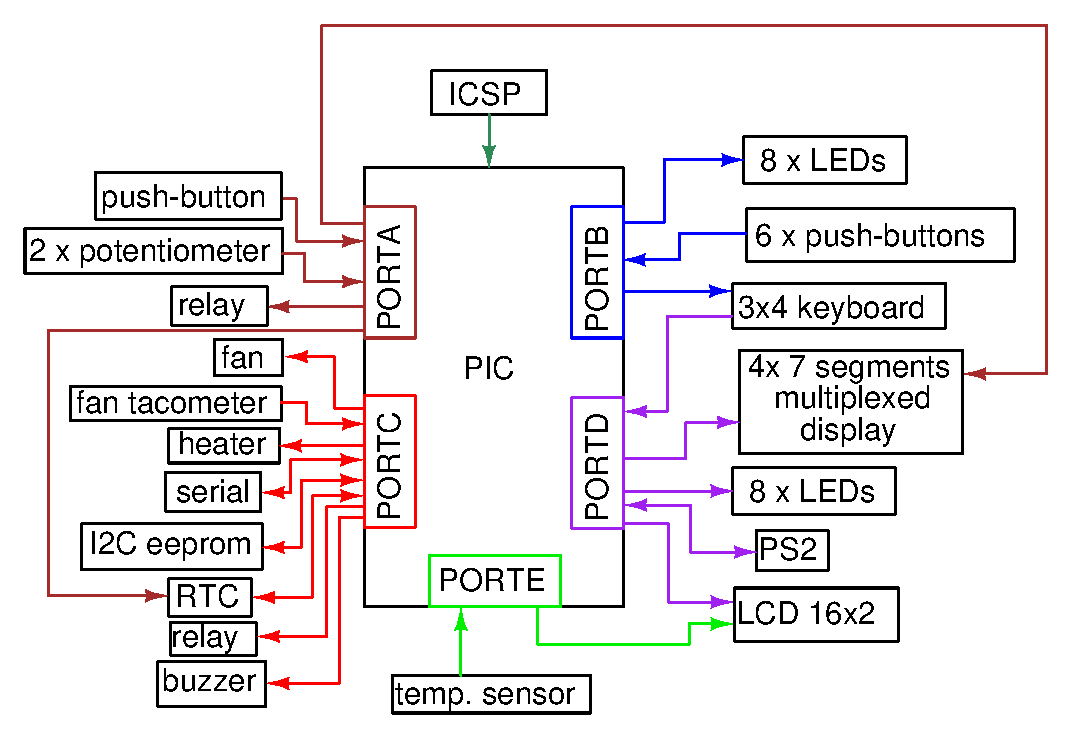
\includegraphics[width=0.85\textwidth]{img/blocks_p4.eps} 
\end{figure} 


\begin{figure}[H]
\center
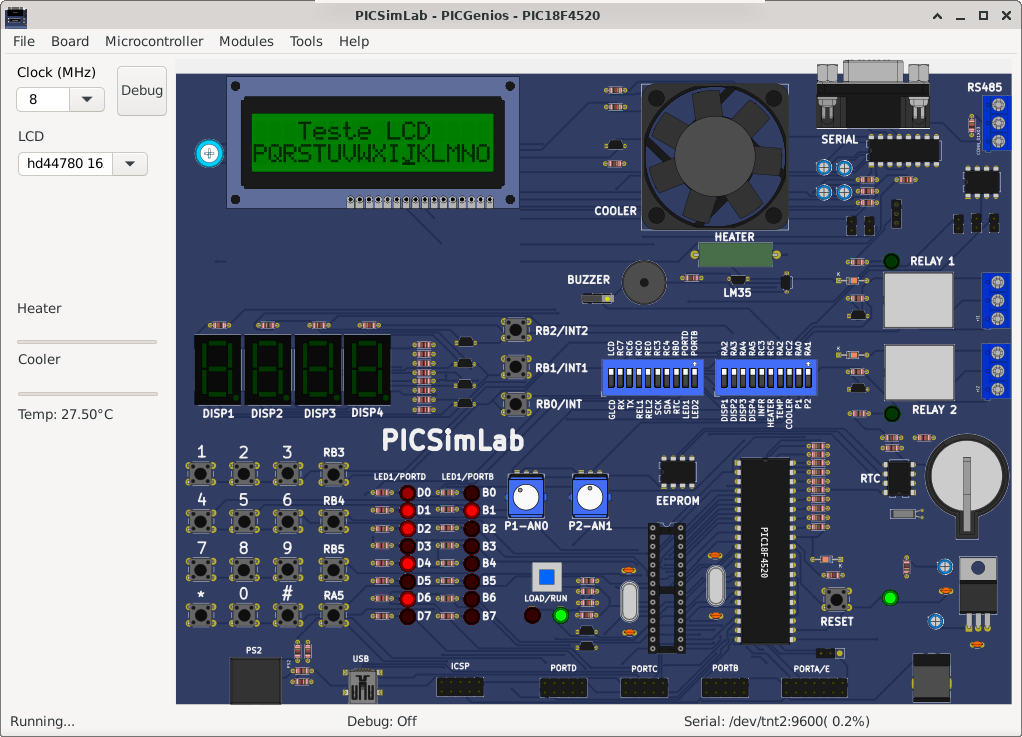
\includegraphics[width=0.99\textwidth]{img/picsimlab4.png} 
\end{figure} 

\hrefb{pdf/board4.pdf}{Board PICGenios schematics}.\vspace{0.5cm}

The code examples can be loaded in PICSimLab menu \textbf{Help->Examples}.

The source code of board PICGenios examples using 
\href{http://www.microchip.com/mplabx}{MPLABX and XC8} compiler are in the link: 
\href{https://lcgamboa.github.io/picsimlab_examples/board_PICGenios.html}{board\_PICGenios}.


\section{PQDB}

The PQDB board is an opensource/openhardware project, more info at \href{https://github.com/projetopqdb/}{https://github.com/projetopqdb/}.
It was developed to be used with arduino/freedom boards, but adapted to use the microcontroller PIC18F4520 of 
\href{https://github.com/lcgamboa/picsim}{picsim} on PICSImLab.

\begin{figure}[H]
\center
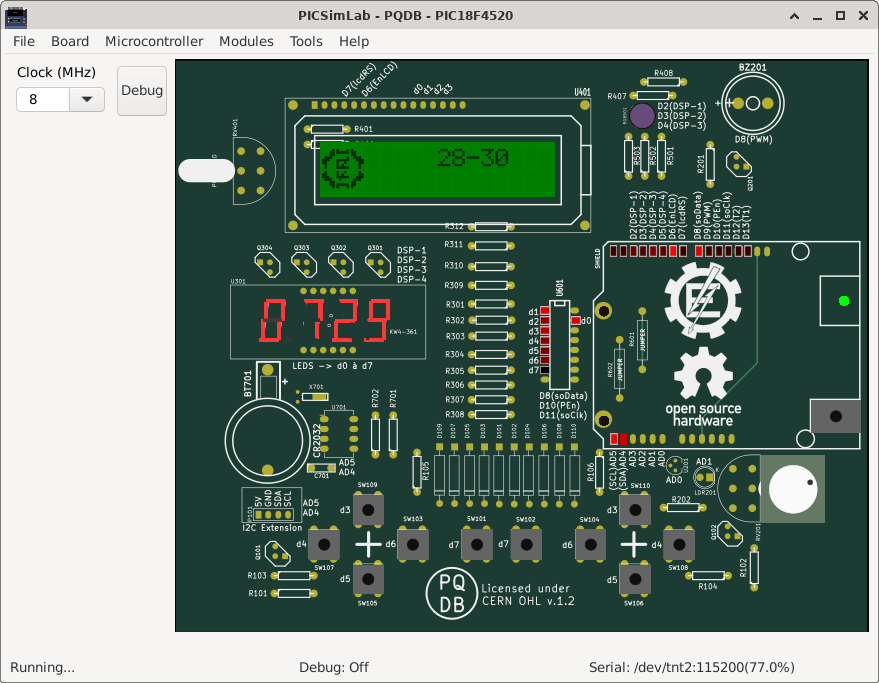
\includegraphics[width=0.99\textwidth]{img/board_PQDB.png} 
\end{figure} 

\href{https://lcgamboa.github.io/picsimlab_examples/board_PQDB.html}{Examples}


\section{Arduino Uno}

It emulates the Arduino Uno development board that uses one ATMEGA328P microcontroller of \href{https://github.com/buserror/simavr}{simavr}.

\begin{figure}[H]
\center
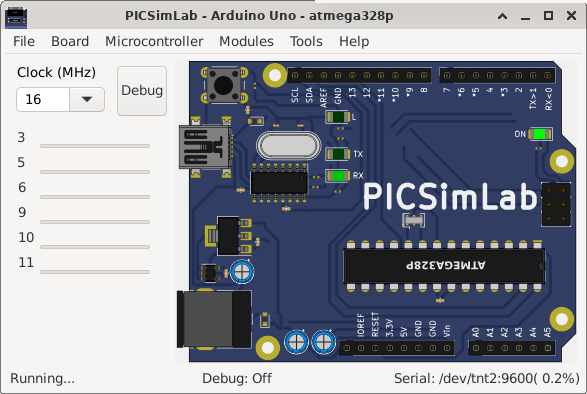
\includegraphics[width=0.80\textwidth]{img/picsimlab5.png} 
\end{figure} 

\href{https://www.arduino.cc/en/uploads/Main/Arduino_Uno_Rev3-schematic.pdf}{Board Arduino Uno schematics}.\vspace{0.5cm}

The code examples can be loaded in PICSimLab menu \textbf{Help->Examples}.

The source code of board Arduino Uno examples using the 
\href{https://www.arduino.cc/en/Main/Software}{Arduino IDE with avr-gcc} are in the link: 
\href{https://lcgamboa.github.io/picsimlab_examples/board_Arduino_Uno.html}{board\_Arduino\_Uno}.

More information about the Arduino in \href{https://www.arduino.cc/}{www.arduino.cc}

\section{Franzininho DIY}

The Franzininho DIY board is an openhardware project, more info at \href{https://franzininho.com.br/}{https://franzininho.com.br/}.
It was developed to be used with the microcontroller ATtiny85 of 
of \href{https://github.com/buserror/simavr}{simavr}.

\begin{figure}[H]
\center
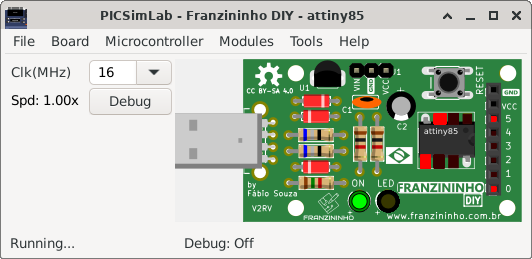
\includegraphics[width=0.7\textwidth]{img/board_Franzininho_DIY.png} 
\end{figure} 

\href{https://lcgamboa.github.io/picsimlab_examples/board_Franzininho_DIY.html}{Examples}


\section{uCboard}

It is a generic board only with reset, serial and crystal circuits and support to multiple microcontrollers 
(initially C51, Z80 and STM8S103 )of \href{http://mazsola.iit.uni-miskolc.hu/\%7edrdani/embedded/ucsim/}{uCsim}.

\begin{figure}[H]
\center
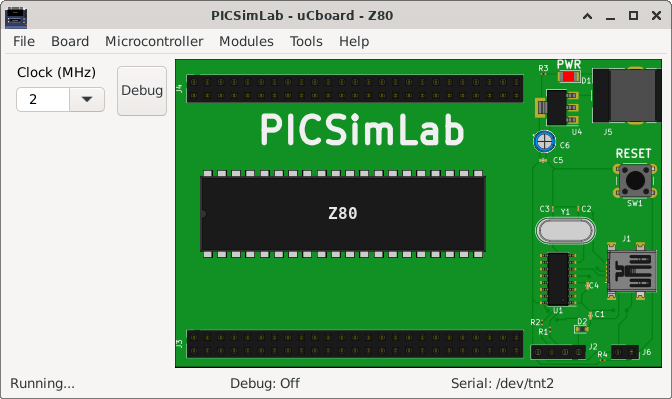
\includegraphics[width=0.7\textwidth]{img/uCboard.png} 
\end{figure} 

\href{https://lcgamboa.github.io/picsimlab_examples/board_uCboard.html}{Examples}
